\documentclass[]{article}
\usepackage{geometry}
\usepackage{amsthm}
\usepackage{mathtools}
\usepackage{amsfonts}
\usepackage{tikz}
\usepackage{eurosym}
\DeclareRobustCommand{\officialeuro}{%
	\ifmmode\expandafter\text\fi
	{\fontencoding{U}\fontfamily{eurosym}\selectfont e}}
\usepackage{caption}
\usepackage{subcaption}
\usetikzlibrary{matrix}

\newtheorem{definition}{Definition}[section]
\newtheorem{theorem}{Theorem}[section]
\newtheorem{lemma}[theorem]{Lemma}



%opening
\title{Verifying Featured Transition Systems using Variability Parity Games}
\author{Sjef van Loo}

\begin{document}

\maketitle

\tableofcontents

\section{Introduction}
Model verification techniques can be used to improve the quality of software. These techniques require the behaviour of the software to be modelled, after which the model can checked to verify that it behaves conforming to some requirement. Different languages are proposed and well studied to express these requirements, examples are LTL, CTL, CTL* and $\mu$-calculus (TODO: cite). Once the behaviour is modelled and the requirement is expressed in some language we can use modal checking techniques to determine if the model satisfies the requirement.

These techniques are well suited to model and verify the behaviour of a single software product. However software systems can be designed to have certain parts enabled or disabled. This gives rise to many software products that all behave very similar but not identical, such a collection is often called a \textit{product family}. The differences between the products in a product family is called the \textit{variability} of the family. A family can be verified by using the above mentioned techniques to verify every single product independently. However this approach does not use the similarities in behaviour of these different products, an approach that would make use of the similarities could potentially be a lot more efficient.

\textit{Labelled transition systems} (LTSs) are often used to model the behaviour of a system, while it can model behaviour well it can't model variability. Efforts to also model variability include I/O automata, modal transition systems and \textit{featured transition systems} (FTSs) (TODO: cite). Specifically the latter is well suited to model all the different behaviours of the software products as well as the variability of the entire system in a single model.

Efforts have been made to verify requirements for entire FTSs, as well as to be able to reason about features. Notable contributions are fLTL, fCTL and fNuSMV (TODO: cite). However, as far as we know, there is no technique to verify an FTS against a $\mu$-calculus formula. Since the modal $\mu$-calculus is very expressive, it subsumes other temporal logics like LTL, CTL and CTL*, this is desired. In this thesis we will introduce a technique to do this. We first look at LTSs, the modal $\mu$-calculus and FTSs. Next we will look at an existing technique to verify an LTS, namely solving \textit{parity games}, as well as show how this technique can be used to verify an FTS by verifying every software product it describes independently. An extension to this technique is then proposed, namely solving \textit{variability parity games}. We will formally define variability parity games and prove that solving them can be used to verify FTSs.

\section{Verifying transition systems}
We first look at labelled transition systems (LTSs) and the modal $\mu$-calculus and what it means to verify an LTS. The definition below are derived from \cite{Groote}.
\begin{definition}
	\label{def_lts}A labelled transition system (LTS) is a tuple $M = (S, Act, trans, s_0)$, where:
	\begin{itemize}
		\item $S$ is a set of states,
		\item $Act$ a set of actions,
		\item $trans \subseteq S \times Act \times S$ is the transition relation with $(s,a,s') \in trans$ denoted by $s \xrightarrow a s'$,
		\item $s_0 \in S$ is the initial state.
	\end{itemize}
\end{definition}
Consider the example in figure \ref{fig:coffeemachinebasiceurolts} (directly taken from \cite{FamBasedModelCheckingWithMCRL2}) of a coffee machine where we have two actions: ins (insert coin) and std (get standard sized coffee).\\
\begin{figure}[h]
	\centering
	\includegraphics[scale=0.5]{Examples/CoffeeMachine/BasicEuroLTS}
	\caption[Coffee machine LTS]{Coffee machine LTS $C$}
	\label{fig:coffeemachinebasiceurolts}
\end{figure}


\begin{definition}
	\label{def_mu_syntax}
	A modal $\mu$-calculus formula over the set of actions $Act$ and a set of variables $\mathcal{X}$ is defined by
	\[ \varphi = \top\ |\ \bot\ |\ X\ |\ \varphi \vee \varphi\ |\ \varphi \wedge \varphi\ |\ \langle a \rangle \varphi\ |\ [a]\varphi\ |\ \mu X.\varphi\ |\ \nu X.\varphi \]
	with $a \in Act$ and $X \in \mathcal{X}$. 
	
	
	No negations in the language because negations can be pushed inside to the propositions, ie. the $\top$ and $\bot$ elements.
\end{definition}
The modal $\mu$-calculus contains boolean constants $\top$ and $\bot$, propositional operators $\vee$ and $\wedge$, modal operators $\langle \, \rangle$ and $[ \, ]$ and fixpoint operators $\mu$ and $\nu$. A formula is closed when variables only occur in the scope of a fixpoint operator for that variable.

A modal $\mu$-calculus formula can be interpreted with an LTS, this results in a set of states for which the formula holds.
\begin{definition}
	\label{def_mu_sem} For LTS $(S, Act, trans, s_0)$ we inductively define the interpretation of a modal $\mu$-calculus formula $\varphi$, notation
	$[\![ \varphi ]\!]^\eta$, where $\eta : \mathcal{X} \rightarrow \mathcal{P}(S)$ is a logical variable valuation, as a set of states
	where $\varphi$ is valid, by:
	\begin{align*}
	&[\![ \mathit{\top} ]\!]^\eta &&= S\\
	&[\![ \mathit{\bot} ]\!]^\eta &&= \emptyset\\
	&[\![ \varphi_1 \wedge \varphi_2 ]\!]^\eta &&= [\![ \varphi_1 ]\!]^\eta \cap [\![ \varphi_2 ]\!]^\eta \\
	&[\![ \varphi_1 \vee \varphi_2 ]\!]^\eta &&= [\![ \varphi_1 ]\!]^\eta \cup [\![ \varphi_2 ]\!]^\eta\\
	&[\![ \langle a \rangle \varphi ]\!]^\eta &&= \{s \in S|\exists_{s' \in S} s \xrightarrow {a} s' \wedge s' \in [\![ \varphi ]\!]^\eta\}\\
	&[\![ [ a ] \varphi ]\!]^\eta &&= \{s \in S|\forall_{s' \in S} s \xrightarrow {a} s' \implies s' \in [\![ \varphi ]\!]^\eta\}\\
	&[\![ \mu X. \varphi ]\!]^\eta &&= \bigcap_{f \subseteq S}\{f | f = [\![ \varphi ]\!]^{\eta[X:=f]}\}\\
	&[\![ \nu X. \varphi ]\!]^\eta &&= \bigcup_{f \subseteq S}\{f | f = [\![ \varphi ]\!]^{\eta[X:=f]}\}\\
	&[\![ X ]\!]^\eta &&= \eta(X)
	\end{align*}
\end{definition}

Given closed formula $\varphi$, LTS $M = (S, Act, trans, s_0)$ and $s \in S$ we write $(M,s) \models \varphi$ iff $s \in [\![ \varphi ]\!]^\eta$ for $M$, we say that formula $\varphi$ holds for $M$ in state $s$. If formula $\varphi$ holds for $M$ in the initial state we say that formula $\varphi$ holds for $M$ and write $M \models \varphi$.

Again consider the coffee machine example (figure \ref{fig:coffeemachinebasiceurolts}) and formula $\varphi = \nu X. \mu Y. ([ins]Y \wedge [std] X)$ (taken from \cite{FamBasedModelCheckingWithMCRL2}) which states that action std must occur infinitely often over all runs. Obviously this holds for the coffee machine, therefore we have $C \models \varphi$.

\subsection{Featured transition systems}
A featured transition system extends the LTS definition to express variability. It does so by introducing \textit{features} and \textit{products} into the definition. Features are options that can be enabled or disabled for the system. A product is a feature assignments, ie. a set of features that is enabled for that product. Not a products are valid, some features might be mutually exclusive and some features might always be required. To express products one can use feature diagrams as explained in \cite{Classen2013FeaturedTS}. Feature diagrams offer a nice way of expressing which feature assignments are valid, but since they offer just that we simply represent the valid products with a set of feature assignments. Finally FTSs guards every transition with a boolean expression over the set of features. We have the following definition, based on \cite{Classen2013FeaturedTS}:
\begin{definition}
	\label{def_fts}A featured transition system (FTS) is a tuple $M = (S, Act, trans, s_0, N, P, \gamma)$, where:
	\begin{itemize}
		\item $S, Act, trans, s_0$ are defined as in an LTS,
		\item $N$ is a non-empty set of features,
		\item $P \subseteq \mathcal{P}(N)$ is a set of products, ie. feature assignments, that are valid,
		\item $\gamma : trans \rightarrow \mathbb{B}(N)$ is a total function, labelling each transition with a boolean expression over the features. A product $p \in \mathcal{P}(N)$ satisfying the boolean expression of transition $t$ is denoted by $p \models \gamma(t)$, $\gamma(t)(p) = 1$ or $p \in [\![\gamma(t)]\!]$. The boolean expression that is satisfied by any feature assignment is denoted by $\top$, ie $p \models \top$ for any $p$.
		
		A transition $s \xrightarrow a s'$ and $\gamma((s,a,s')) = f$ is denoted by $s \xrightarrow {a | f} s'$. 
	\end{itemize}
\end{definition}
\begin{figure}[h]
\centering
\includegraphics[scale=0.5]{Examples/CoffeeMachine/FTS}
\caption[Coffee machine LTS]{Coffee machine FTS $C$}
\label{fig:coffeemachinefts}
\end{figure}

Consider the example in figure \ref{fig:coffeemachinefts} (directly taken from \cite{FamBasedModelCheckingWithMCRL2}) which shows an FTS for a coffee machine For this example we have two features $N = \{\$, \officialeuro\}$ and two valid products $P = \{\{\$\},\{\officialeuro\}\}$.

An FTS expresses they behaviour of multiple products, we can derive the behaviour of a single product by simply removing all the transitions from the FTS for which the product doesn't satisfy the feature expression guarding the transition. We call this a \textit{projection} (\cite{Classen2013FeaturedTS}).

\begin{definition}
	\label{def_fts_proj}
	The projection of an FTS $M = (S, Act, trans, s_0, N, P, \gamma)$ to a product $p \in P$, noted $M_{|p}$, is the LTS $M'=(S,Act,trans', s_0)$, where $trans' = \{t \in trans\ |\ p \models \gamma(t)\}$.
\end{definition}
The coffee machine example can be projected to its two products, which results in the LTSs in figure \ref{fig:cofeemachineftsproj}.
\begin{figure}[h]
	\centering
	\begin{subfigure}{.5\textwidth}
		\centering
		\includegraphics[width=1\linewidth]{Examples/CoffeeMachine/FTSProjDollar}
		\caption[$C_{|\{\$\}}$]{$C$ projected to the dollar product: $C_{|\{\$\}}$}
		\label{fig:coffeemachineftsprojdollar}
	\end{subfigure}%
	\begin{subfigure}{.5\textwidth}
		\centering
		\includegraphics[width=1\linewidth]{Examples/CoffeeMachine/FTSProjEuro}
		\caption[$C_{|\{\$\}}$]{$C$ projected to the euro product: $C_{|\{\officialeuro\}}$}
		\label{fig:coffeemachineftsprojeuro}
	\end{subfigure}
	\caption{Projections of the coffee machine FTS}
	\label{fig:cofeemachineftsproj}
\end{figure}

We want to verify the FTS against a modal $\mu$-calculus formula $\varphi$. That is, we want to find out for which products in the FTS its projection satisfies $\varphi$. Formally, given FTS $M = (S, Act, trans, s_0, N, P, \gamma)$ and modal $\mu$-calculus formula $\varphi$ we want to find $P_s \subseteq P$ such that:
\begin{itemize}
	\item for every $p \in P_s$ we have $M_{|p} \models \varphi$ and
	\item for every $p \in P \backslash P_s$ we have $M_{|p} \not\models \varphi$.
\end{itemize}
Furthermore a counterexample for every $p \in P \backslash P_s$ is preferred.

\section{Verification using parity games}
Verifying LTSs against a modal $\mu$-calculus formula can be done by solving a parity game. This is done by translating an LTS in combination with a formula to a parity game, the solution of the parity game provides the information needed to conclude if the model satisfies the formula. This relation is depicted in figure \ref{fig:ltsverificationusingpg}. This technique is well known and well studied, in this section we will first look at parity games, the translation from LTS and formula to a parity game and finally what we can do with this technique to verify FTS.
\begin{figure}[h]
	\centering
	\includegraphics[scale=0.5]{Diagrams/LTSVerificationUsingPG}
	\caption[LTS verification using PG]{LTS verification using PG}
	\label{fig:ltsverificationusingpg}
\end{figure}

\subsection{Parity games}
\begin{definition}
	\label{def_PG}\cite{Bradfield2018}
	A parity game (PG) is a tuple $(V, V_0, V_1, E, \rho)$, where:
	\begin{itemize}
		\item $V = V_0 \cup V_1$ and $V_0 \cap V_1 = \emptyset$,
		\item $V_0$ is the set of vertices owned by player $0$,
		\item $V_1$ is the set of vertices owned by player $1$, 
		\item $E \subseteq V \times V$ is the edge relation,
		\item $\rho :  V \rightarrow \mathbb{N}$ is a priority assignment.
	\end{itemize}
\end{definition}
We write $\alpha \in \{0,1\}$ to denote an arbitrary player. We write $\overline{\alpha}$ to denote $\alpha$'s opponent, ie. $\overline{0} = 1$ and $\overline{1} = 0$.

A parity game is played by players 0 and 1. A play starts with placing a token on vertex $v \in V$. Player $\alpha$ moves the token if the token is on a vertex owned by $\alpha$, ie. $v \in V_\alpha$. The token can be moved to $w \in V$, with $(v,w) \in E$. A series of moves results in a sequence of vertices, called path. For path $\pi$ we write $\pi_i$ to denote the $i^{\text{th}}$ vertex in path $\pi$. A play ends when the token is on vertex $v \in V_\alpha$ and $\alpha$ can't move the token anywhere, in this case player $\overline{\alpha}$ wins the play. If the play results in an infinite path $\pi$ then we determine the highest priority that occurs infinitely often in this path, formally
\[ \max\{ p \ |\ \forall_j \exists_i j < i \wedge p = \rho(\pi_i) \}\] 
If the highest priority is odd then player $1$ wins, if it is even player $0$ wins.
\begin{figure}[h]
	\centering
	\includegraphics[scale=0.3]{Examples/SimplePG/PG}
	\caption[Parity game example]{Parity game example}
	\label{fig:simplepgpg}
\end{figure}

Figure \ref{fig:simplepgpg} shows an example of a parity game. We usually depict the vertices owned by player $0$ by diamonds and vertices owned by player $1$ by boxes, the priority is depicted inside the vertices. If the game starts by placing a token on $v_1$ we can consider the following exemplary paths:
\begin{itemize}
	\item $\pi = v_1v_3v_5$ is won by player $1$ since player $0$ can't move at $v_5$.
	\item $\pi = (v_1v_2)^\omega$ is won by player $1$ since the highest priority occurring infinitely often is 3.
	\item $\pi = v_1v_3(v_4)^\omega$ is won by player $0$ since the highest priority occurring infinitely often is $0$.
\end{itemize}


A strategy for player $\alpha$ is a function $\sigma : V^*V_\alpha \rightarrow V$ that maps a path ending in a vertex owned by player $\alpha$ to the next vertex. Parity games are positionally determined \cite{Bradfield2018}, therefore a strategy $\sigma: V_\alpha \rightarrow V$ that maps the current vertex to the next vertex is sufficient. 

A strategy $\sigma$ for player $\alpha$ is winning from vertex $v$ if and only if any play that results from following $\sigma$ results in a win for player $\alpha$. The graph can be divided in two partitions $W_0 \subseteq V$ and $W_1 \subseteq V$, called winning sets. If and only if $v \in W_\alpha$ then player $\alpha$ has a winnings strategy from $v$. Every vertex in the graph is either in $W_0$ or $W_1$ \cite{Bradfield2018}. Furthermore finite parity games are decidable \cite{Bradfield2018}.
\subsection{Creating parity games}

\subsection{FTSs and parity games}

\section{Featured parity games}







Before we can define variability parity games we first define \textit{featured parity games} (FPG), featured parity games extend the definition of parity games to capture the variability represented in an FTS. It uses the same concepts as FTSs: features, products and a function that guards edges. In this section we will introduce the definition of FPGs and show that solving them answers the verification questions for FTS: For which products in the FTS does its projection satisfy $\varphi$?

First we introduce the definition of an FPG:
\begin{definition}
	\label{def_FPG}
	A featured parity game (FPG) is a tuple $(V,V_0, V_1, E, \Omega, N, P, \gamma)$, where:
	\begin{itemize}
		\item $V = V_0 \cup V_1$ and $V_0 \cap V_1 = \emptyset$,
		\item $V_0$ is the set of vertices owned by player $0$,
		\item $V_1$ is the set of vertices owned by player $1$, 
		\item $E \subseteq V \times V$ is the edge relation,
		\item $\Omega :  V \rightarrow \mathbb{N}$ is a priority assignment,
		\item $N$ is a non-empty set of features,
		\item $P \subseteq \mathcal{P}(N)$ is a non-empty set of products, ie. feature assignments, for which the game can be played,
		\item $\gamma : E \rightarrow \mathbb{B}(N)$ is a total function, labelling each edge with a Boolean expression over the features.
	\end{itemize}
\end{definition}
An FPG is played similarly to a PG, however the game is played for a specific product $p \in P$. Player $\alpha$ can only move the token from $v \in V_\alpha$ to $w \in V$ if $(v,w) \in E$ and $p \models \gamma(v,w)$.

A game played for product $p \in P$ results in winnings sets $W_0^p$ and $W_1^p$, which are defined similar to the $W_0$ and $W_1$ winning sets for parity games.

An FPG can simply be projected to a product $p$ by removing the edges that are not satisfied by $p$.
\begin{definition}
	\label{def_FPG_proj}
	The projection from FPG $G = (V,V_0, V_1, E, \Omega, N, P, \gamma)$ to a product $p \in P$, noted $G_{|p}$, is the parity game $(V,V_0,V_1, E', \Omega)$ where $E' = \{ e \in E\ |\ p \models \gamma(e) \}$.
\end{definition}

Playing FPG $G$ for a specific product $p\in P$ is the same as playing the PG $G_{|p}$. Any path that is valid in $G$ for $p$ is also valid in $G_{|p}$ and vice versa. Therefore the strategies are also interchangeable, furthermore the winning sets $W_\alpha$ for $G_{|p}$ and $W_\alpha^p$ for $G$ are identical. Since parity games are positionally determined so are FPGs. Similarly, since finite parity games are decidable, so are finite FPGs.

We say that an FPG is solved when the winning sets for every valid product in the FPG are determined.
\subsubsection{Creating featured parity games}
An FPG can be created from an FTS in combination with a model $\mu$-calculus formula. We translate an FTS to an FPG by first creating a PG from the transition system as if there were no transition guards, next we apply the same guards to the FPG as are present in the FTS for edges that originate from transitions. The features and valid products in the FPG are identical to those in the FTS.
\begin{definition}
	\label{def_FTS2FPG}
	$FTS2FPG(M, \varphi)$ converts FTS $M = (S, Act, trans, s_0, N, P, \gamma)$ and closed formula $\varphi$ to FPG $(V, V_0, V_1, E, \Omega, N, P, \gamma')$.
	
	We have $(V, V_0, V_1, E, \Omega) = \textit{LTS2PG}((S, Act, trans, s_0), \varphi$) and
	\[ \gamma'((s, \psi),(s', \psi')) = \begin{cases}
	\gamma(s,a,s') & \text{if }\psi = \langle a \rangle \psi'\text{ or }\psi = [a]\psi' \\
	\top & \text{otherwise}
	\end{cases}\]
\end{definition}
Consider our working example which we extend to an FTS depicted in figure \ref{fig:exverfts}, for this example we have features $N = \{f, g\}$ and products $P = \{\emptyset, \{f\},\{f,g\}\}$.

\begin{figure}[h]
	\centering
	\includegraphics[scale=0.3]{Examples/ExamleVerification/FPG}
	\caption[FPG for $M$ and $\varphi$]{FPG for $M$ and $\varphi$}
	\label{fig:exverfpg}
\end{figure}
We can translate this FTS with formula $\varphi = \mu X. ([a] X \vee \langle b \rangle \top)$ to an FPG depicted in figure \ref{fig:exverfpg}. As we can see from the FTS if feature $f$ is enabled and $g$ is disabled then we have an infinite path of $a$'s where $b$ is never enabled, therefore $\varphi$ doesn't hold for $M_{|\{f\}}$. If $g$ is enabled however we can always do a $b$ so $\varphi$ holds for $M_{|\{f,g\}}$. As we have seen $\varphi$ does hold for $M_{|\emptyset}$. For the product $\emptyset$ we have the same winning set as before:
\begin{align*}
W_0^\emptyset = \{& (s_1, \mu X.\phi),\\
& (s_1, [a](\mu X.\phi) \vee \langle b \rangle \top),\\
& (s_1, [a](\mu X.\phi)),\\
& (s_1, \top),\\
& (s_2, \mu X.\phi),\\
& (s_2, [a](\mu X.\phi) \vee \langle b \rangle \top),\\
& (s_2, [a](\mu X.\phi)),\\
& (s_2, \langle b \rangle \top),\\
& (s_2, \top)
\}\\
W_1^\emptyset = \{& (s_1, \langle b \rangle \top )\}
\end{align*}
In the FPG we can see that if $f$ is enabled and $g$ is disabled then player $1$ can move the token from $(s_1, [a]X)$ to $(s_1,X)$. This results in player $0$ either moving the token to $(s_1, \langle b \rangle \top)$ and losing or an infinite path where $1$ occurs infinitely often which is also player $1$ wins. For product $\{f\}$ we have winning sets:
\begin{align*}
W_0^{\{f\}} = \{
& (s_1, \top),\\
& (s_2, \mu X.\phi),\\
& (s_2, [a](\mu X.\phi) \vee \langle b \rangle \top),\\
& (s_2, \langle b \rangle \top),\\
& (s_2, \top)
\}\\
W_1^{\{f\}} = \{& (s_1, \mu X.\phi),\\
& (s_1, [a](\mu X.\phi) \vee \langle b \rangle \top),\\
& (s_1, [a](\mu X.\phi)),\\
& (s_1, \langle b \rangle \top ),\\
& (s_2, [a](\mu X.\phi))\}
\end{align*}
However if $g$ is also enabled then player $0$ wins in $(s_1, \langle b \rangle \top)$, thus giving the following winning sets:
\begin{align*}
W_0^{\{f,g\}} = \{& (s_1, \mu X.\phi),\\
& (s_1, [a](\mu X.\phi) \vee \langle b \rangle \top),\\
& (s_1, [a](\mu X.\phi)),\\
& (s_1, \langle b \rangle \top ),\\
& (s_1, \top),\\
& (s_2, \mu X.\phi),\\
& (s_2, [a](\mu X.\phi) \vee \langle b \rangle \top),\\
& (s_2, [a](\mu X.\phi)),\\
& (s_2, \langle b \rangle \top),\\
& (s_2, \top)
\}\\
W_1^{\{f,g\}} = \{\}
\end{align*}

In the next section we will show how the winning sets relate to the model verification question.


\subsubsection{FTS verification using featured parity games}
We can create an FPG from an FTS and project it to a product, resulting in a PG, this is shown in the following diagram:\\
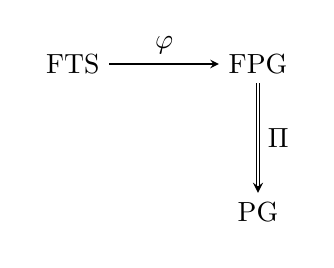
\begin{tikzpicture}
\matrix (m) [matrix of math nodes,row sep=4em,column sep=4em,minimum width=2em]
{
	\text{FTS} & \text{FPG} \\
	\  & \text{PG} \\};
\path[-stealth]
(m-1-1)
edge node [above] {$\varphi$} (m-1-2)

(m-1-2) edge [double] node [right] {$\Pi$} (m-2-2)
;
\end{tikzpicture}\\
Earlier we saw that we could also derive a PG by projecting the FTS to a product and then translation the resulting LTS to a PG, depicted by the following diagram:
\\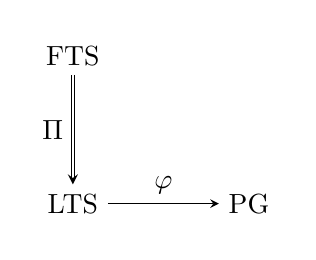
\begin{tikzpicture}
\matrix (m) [matrix of math nodes,row sep=4em,column sep=4em,minimum width=2em]
{
	\text{FTS} \\
	\text{LTS} & \text{PG} \\};
\path[-stealth]
(m-1-1) edge [double] node [left] {$\Pi$} (m-2-1)
(m-2-1.east|-m-2-2) edge node [above] {$\varphi$}
(m-2-2)
;
\end{tikzpicture}\\
We will now show that the resulting parity games are identical.
\begin{theorem}
	\label{the_PGsubPGA} Given:
	\begin{itemize}
		\item FTS $M = (S,Act, trans, s_0, N, P, \gamma)$,
		\item a closed modal mu-calculus formula $\varphi$,
		\item a product $p \in P$
	\end{itemize}
	it holds that the parity games LTS2PG($M_{|p}, \varphi$) and FTS2FPG($M, \varphi$)$_{|p}$  are identical.
	\begin{proof}
		Let $G^F = (V^F, V_0^F, V_1^F, E^F, \Omega^F, N, P, \gamma') = FTS2FPG(M, \varphi)$, using definition \ref{def_FTS2FPG}, and $G^F_{|p} = (V^F, V_0^F, V_1^F, {E^F}', \Omega^F)$, using definition \ref{def_FPG_proj}. Furthermore we have $M_{|p} = (S, Act, trans', s_0)$ and we let $G = (V, V_0, V_1, E, \Omega) =  LTS2PG(M_{|p}, \varphi)$. We depict the different transition systems and games in the following diagram.
		
		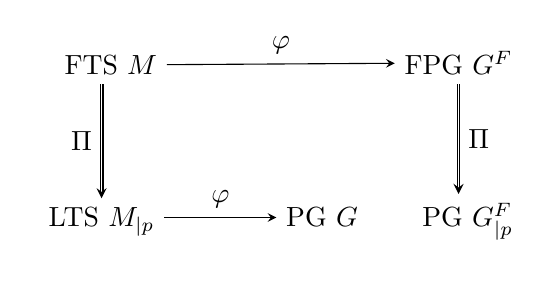
\begin{tikzpicture}
		\matrix (m) [matrix of math nodes,row sep=4em,column sep=1em,minimum width=2em]
		{
			\text{\ \ FTS }M & \  &\ & \text{FPG } G^F  \\
			\text{LTS }M_{|p} & \ & \text{PG } G & \text{\ \ PG }G_{|p}^F \\};
		\path[-stealth]
		(m-1-1) edge [double] node [left] {$\Pi$} (m-2-1)
		edge node [above] {$\varphi$} (m-1-4)
		(m-2-1.east|-m-2-3) edge node [above] {$\varphi$}
		(m-2-3)
		(m-1-4) edge [double] node [right] {$\Pi$} (m-2-4);
		\end{tikzpicture}\\
		We will prove that $G = G_{|p}^F$. We first note that game $G$ is created by 
		\[  (V, V_0, V_1, E, \Omega) = LTS2PG((S, Act, trans', s_0),\varphi) \]
		and the vertices, edges and priorities of game $G^F$ are created by 
		\[ (V^F, V_0^F, V_1^F, E^F, \Omega^F) = LTS2PG((S,Act, trans, s_0), \varphi)\]
		Using the definition of LTS2PG (\ref{def_LTS2PG}) we find that the vertices and the priorities only depend on the states in $S$ and the formula $\varphi$, since these are identical in the above two statements we immediately get $V = V^F, V_0 = V_0^F, V_1 = V_1^F$ and $\Omega = \Omega^F$. The vertices and priorities don't change when an FTS is projected, therefore $G_{|p}^F$ has the same vertices and priorities as $G^F$.
		
		Now we are left with showing that $E = {E^F}'$ in order to conclude that that $G = G^F_{|p}$. We will do this by showing $E \subseteq {E^F}'$ and $E \supseteq {E^F}'$.
		
		First let $e \in E$. Note that a vertex in the parity game is represented by a pair of a state and a formula. So we can write $e = ((s,\psi),(s',\psi'))$. To show that $e \in {E^F}'$ we distinguish two cases:
		\begin{itemize}
			\item  If $\psi = \langle a \rangle \psi'$ or $\psi = [a] \psi'$ then there exists an $a \in Act$ such that $(s,a,s') \in trans'$. Using the FTS projection definition (\ref{def_fts_proj}) we get $(s,a,s') \in trans$ and $p \models \gamma(s,a,s')$. Using the FTS2FPG definition (\ref{def_FTS2FPG}) we find that $\gamma'((s,\psi),(s',\psi')) = \gamma(s,a,s')$ and therefore $p \models \gamma'((s,\psi),(s',\psi'))$. Now using the FPG projection definition (\ref{def_FPG_proj}) we find $((s,\psi),(s',\psi')) \in {E^F}'$.
			\item Otherwise the existence of the edge does not depend on the $trans$ parameter and therefore $((s,\psi),(s',\psi')) \in {E^F}'$ if $(s,\psi) \in V^F$, since $V^F = V$ we have $(s,\psi) \in V^F$.
		\end{itemize}
		We can conclude that $E \subseteq {E^F}'$, next we will show $E \supseteq {E^F}'$. Let $e = ((s,\psi),(s',\psi')) \in {E^F}'$. We distinguish two cases:
		\begin{itemize}
			\item If $\psi = \langle a \rangle \psi'$ or $\psi = [a] \psi'$ then there exists an $a \in Act$ such that $(s,a,s') \in trans$. Using the FPG projection definition (\ref{def_FPG_proj}) we get $p \models \gamma'(s,a,s')$. Using the FTS2FPG definition (\ref{def_FTS2FPG}) we get $p \models \gamma(s,a,s')$. Using the FTS projection definition (\ref{def_fts_proj}) we get $(s,a,s') \in trans'$ and therefore $((s,\psi),(s',\psi'))\in E$.
			\item Otherwise the existence of the edge does not depend on the $trans$ parameter and therefore $((s,\psi),(s',\psi')) \in E$ if $(s,\psi) \in V$, since $V^F = V$ we have $(s,\psi) \in V$.
		\end{itemize}
	\end{proof}
\end{theorem}

Having proven this we can visualize the relation between the different games and transition systems in the following diagram:
\\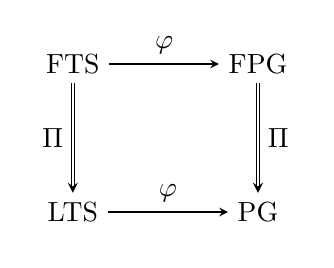
\begin{tikzpicture}
\matrix (m) [matrix of math nodes,row sep=4em,column sep=4em,minimum width=2em]
{
	\text{FTS} & \text{FPG} \\
	\text{LTS} & \text{PG} \\};
\path[-stealth]
(m-1-1) edge [double] node [left] {$\Pi$} (m-2-1)
edge node [above] {$\varphi$} (m-1-2)
(m-2-1.east|-m-2-2) edge node [above] {$\varphi$}
(m-2-2)
(m-1-2) edge [double] node [right] {$\Pi$} (m-2-2)
;
\end{tikzpicture}\\
Finally we prove that solving an FTS, ie. finding winning sets for all products, answers the verification question.
\begin{theorem}
	\label{the_FPG_ver_FTS}
	Given:
	\begin{itemize}
		\item FTS $M = (S, Act, trans, s_0, N, P, \gamma)$,
		\item closed modal mu-calculus formula $\varphi$,
		\item product $p \in P$ and
		\item state $s \in S$
	\end{itemize}
	it holds that $(M_{|p}, s) \models \varphi$ if and only if $(s, \varphi) \in W_0^p$ in $\textit{FTS2FPG}(M, \varphi$).
	\begin{proof}
		The winning set $W_\alpha^p$ is equal to winning set $W_\alpha$ in $\textit{FTS2FPG}(M, \varphi)_{|p}$, for any $\alpha \in \{0,1\}$, using the FPG definition (\ref{def_FPG}). Using theorem \ref{the_PGsubPGA} we find that the game $FTS2FPG(M, \varphi)_{|p}$ is equal to the game $LTS2PG(M_{|p}, \varphi)$, obviously their winning sets are also equal. Using the well studied relation between parity games and LTS verification, stated in theorem \ref{the_LTS_PG_REL}, we know that $(M_{|p}, s) \models \varphi$ if and only if $(s, \varphi) \in W_0$ in game $LTS2PG(M_{|p},\varphi)$. Winning set $W_\alpha^p$ is equal to $W_\alpha$, therefore the theorem holds.
	\end{proof}
\end{theorem}

Revisiting our prior example we can see the theorem in action by noting that $M_{|\emptyset} \models \varphi$ , $M_{|\{f\}} \not\models \varphi$ and $M_{|\{f,g\}} \models \varphi$. This is reflected by the vertex $(s_1, \mu X. [a]X \vee \langle b \rangle \top)$ being present in $W_0^\emptyset$ and $W_0^{\{f,g\}}$ but not in $W_0^{\{f\}}$.

\subsection{Variability parity games}
Next we will introduce \textit{variability parity games} (VPGs). VPGs are very similar to FPGs, however VPGs use configurations instead of features and products to express variability. This gives a syntactically more pleasant representation that is not solely tailored for FTSs. Furthermore in VPGs deadlocks are removed, by doing so VPG plays can only result in infinite paths and no longer in finite paths.

Later we will show the relation between VPGs and FTS verification, which is similar to the relation between FPGs and FTS verification. First we introduce VPGs.

A VPG is played similarly to a PG, however the game is played for a specific configuration $c \in \mathfrak{C}$. Player $\alpha$ can only move the token from $v \in V_\alpha$ to $w \in V$ if $(v,w) \in E$ and $c \in \theta(v,w)$. Furthermore VPGs don't have deadlocks, therefore every play results in an infinite path.

A game played for configuration $c \in \mathfrak{C}$ results in winning sets $W_0^c$ and $W_1^c$, which are defined similar to the $W_0$ and $W_1$ winning sets for parity games.

Solving a VPG means determining winning sets for every configuration in the VPG.
\begin{definition}
	\label{def_VPG_proj} The projection from VPG $G = (V, V_0, V_1, E, \Omega, \mathfrak{C}, \theta)$ to a configuration $c \in \mathfrak{C}$, noted $G_{|c}$, is the parity game $(V, V_0, V_1, E', \Omega)$ where $E' = \{ e\in E\ |\ c \in \theta(e)\}$.
\end{definition}

Playing VPG $G$ for a specific configuration $c \in \mathfrak{C}$ is the same as playing the PG $G_{|c}$. Any path that is valid in $G$ for $c$ is also valid in $G_{|c}$ and vice versa. Therefore the strategies are also interchangeable, furthermore the winning sets $W_\alpha$ for $G_{|c}$ and $W_\alpha^c$ for $G$ are identical. Since parity games are positionally determined so are VPGs. Similarly, since finite parity games are decidable, so are finite VPGs.
\subsubsection{Creating variability parity games}
We will define a translation from an FPG to a VPG. To do so we use the set of valid products as the set of configurations. Furthermore we make the FPG deadlock free, this is done by creating two losing vertices $l_0$ and $l_1$ such that player $\alpha$ loses when the token is in vertex $l_\alpha$. Any vertex that can't move for a configuration will get an edge that is admissible for that configuration towards one of the losing vertices.
\begin{definition}
	\label{def_FPG2VPG}
	FPG2VPG($G^F$) converts FPG $G^F = (V^F, V_0^F, V_1^F, E^F, \Omega^F, N, P, \gamma)$ to VPG $G = (V, V_0, V_1, E, \Omega, \mathfrak{C}, \theta)$.
	
	We define $\mathfrak{C} = P$. We create vertices $l_0$ and $l_1$ and define $V_0 = V_0^F \cup \{l_0\}$, $V_1 = V_1^F \cup \{l_1\}$ and $V = V_0 \cup V_1$.
	
	We construct $E$ by first making $E = E^F$ and adding edges $(l_0, l_0)$ and $(l_1, l_1)$ to $E$. Simultaneously we construct $\theta$ by first making $\theta(e) = \{p \in \mathfrak{C}\ |\ p \models \gamma(e)\}$ for every $e \in E^F$. Furthermore $\theta(l_0,l_0) = \theta(l_1,l_1) = \mathfrak{C}$.
	
	Next, for every vertex $v \in V_\alpha$ with $\alpha = \{0,1\}$, we have $C = \mathfrak{C} \backslash \bigcup \{\theta(v,w)\ |\ (v,w) \in E\}$. If $C \neq \emptyset$ then we add $(v, l_\alpha)$ to $E$ and make $\theta(v,l_\alpha) = C$.
	Finally we have 
	\[ \Omega(v) = \begin{cases}
	1  & \text{if } v = l_0 \\
	0 & \text{if } v = l_1 \\
	\Omega^F(v) &\text{otherwise}
	\end{cases} \]
\end{definition}
Again considering our previous working example we can translate the FPG shown in figure \ref{fig:exverfpg} to the VPG shown in figure \ref{fig:exvevpg}. Where $c_0$ is product $\emptyset$, $c_1$ is $\{f\}$ and $c_2$ is $\{f,g\}$.

\subsubsection{FTS verification using variability parity games}
We have shown in theorem \ref{the_FPG_ver_FTS} that we can use an FPG to verify an FTS. Next we will show that a winning set in the FPG $M$ is the subset of the winning set in the VPG $\textit{FPG2VPG}(M)$.
\begin{theorem}
	\label{the_FPG_sub_VPG}
	Given:
	\begin{itemize}
		\item FPG $G^F = (V^F, V_0^F, V_1^F, E^F, \Omega^F, N, P, \gamma)$,
		\item product $p \in P$
	\end{itemize}
	we have for winning sets $Q_\alpha^{p}$ in $G^F$ and $W_\alpha^{p}$ in $\textit{FPG2VPG}(G^F)$ that $Q_\alpha^{p} \subseteq W_\alpha^{p}$ for any $\alpha \in \{0,1\}$.
	\begin{proof}
		Let $G = (V,V_0,V_1, E, \Omega, \mathfrak{C},\theta) = \textit{FPG2VPG}(G^F)$. Consider finite play $\pi$ that is valid in game $G^F$ for product $p$. We have for every $(\pi_i, \pi_{i+1})$ in $\pi$ that $(\pi_i, \pi_{i+1}) \in E^F$ and $p \models \gamma(\pi_i, \pi_{i+1})$. From the $\textit{FPG2VPG}$ definition (\ref{def_FPG2VPG}) it follows that $(\pi_i, \pi_{i+1}) \in E$ and $p \in \theta(\pi_i, \pi_{i+1})$. So we can conclude that path $\pi$ is also valid in game $G$ for configuration $p$. Since the play is finite the winner is determined by the last vertex $v$ in $\pi$, player $\alpha$ wins such that $v \in V_{\overline{\alpha}}$. Furthermore we know, because the play is finite, that there exists no $(v,w) \in E^F$ with $p \models \gamma(v,w)$. From this we can conclude that $(v, l_{\overline{\alpha}}) \in E$ and $p \in \theta(v, l_{\overline{\alpha}})$. Vertex $l_{\overline{\alpha}}$ has one outgoing edge, namely to itself. So finite play $\pi$ will in game $G^F$ results in an infinite play $\pi(l_{\overline{\alpha}})^\omega$. Vertex $l_{\overline{\alpha}}$ has a priority with the same parity as player $\alpha$, so player $\alpha$ wins the infinite play in $G$ for configuration $p$.
		
		Consider infinite play $\pi$ that is valid in game $G^F$ for product $p$. As shown above this play is also valid in game $G$ for configuration $p$. Since the win conditions of both games are the same the play will result in the same winner.
		
		Consider infinite play $\pi$ that is valid in game $G$ for configuration $p$. We distinguish two cases:
		\begin{itemize}
			\item If $l_\alpha$ doesn't occur in $\pi$ then the path is also valid for game $G^F$ with product $p$ and has the same winner.
			\item If $\pi = \pi'(l_\alpha)^\omega$ with no occurrence of $l_\alpha$ in $\pi'$ then the winner is player $\overline{\alpha}$. The path $\pi'$ is valid for game $G^F$ with product $p$. Let vertex $v$ be the last vertex of $\pi'$. Since $(v, l_\alpha) \in E$ and $p \in \theta(v,l_\alpha)$ we know that there is no $(v,w) \in E^F$ with $p \models \gamma(v,w)$ and that vertex $v$ is owned by player $\alpha$. So in game $G^F$ player $\alpha$ can't move at vertex $v$ and therefore loses the game (in which case the winner is also $\overline{\alpha}$).
		\end{itemize}
		
		We have shown that every path (finite or infinite) in game $G^F$ with product $p$ can be played in game $G$ with configuration $p$ and that they have the same winner. Furthermore every infinite path in game $G$ with configuration $p$ can be either played as an infinite path or the first part of the path can be played in $G^F$ with product $p$ and they have the same winner. From this we can conclude that the theorem holds.
	\end{proof}
\end{theorem}
We can conclude the diagram depicting the relation between the different games and transition systems:\\
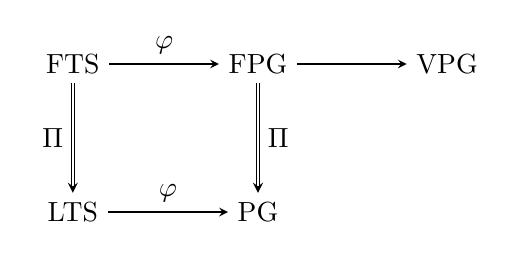
\begin{tikzpicture}
\matrix (m) [matrix of math nodes,row sep=4em,column sep=4em,minimum width=2em]
{
	\text{FTS} & \text{FPG} & \text{VPG} \\
	\text{LTS} & \text{PG} \\};
\path[-stealth]
(m-1-1) edge [double] node [left] {$\Pi$} (m-2-1)
edge node [above] {$\varphi$} (m-1-2)
(m-2-1.east|-m-2-2) edge node [above] {$\varphi$}
(m-2-2)
(m-1-2) edge [double] node [right] {$\Pi$} (m-2-2)
edge (m-1-3);
\end{tikzpicture}\\
Finally we show that solving VPGs, ie. finding the winning sets for all configurations, can be used to verify FTSs.
\begin{theorem}
	\label{the_VPG_ver_FTS}
	Given:
	\begin{itemize}
		\item FTS $M = (S, Act, trans, s_0, N, P, \gamma)$,
		\item closed modal mu-calculus formula $\varphi$,
		\item product $p \in P$ and
		\item state $s \in S$
	\end{itemize}
	it holds that $(M_{|p}, s) \models \varphi$ if and only if $(s, \varphi) \in W_0^{p}$ in $\textit{FPG2VPG}(\textit{FTS2FPG}(M, \varphi))$.
	\begin{proof}
		Let $W_0^{p}$ and $W_1^{p}$ denote the winning sets for game $\textit{FPG2VPG}(\textit{FTS2FPG}(M, \varphi))$. And $Q_0^{p}$ and $Q_1^{p}$ denote the winning sets for game $\textit{FTS2FPG}(M, \varphi)$.
		
		Using theorem \ref{the_FPG_ver_FTS} we find that $(M_{|p}, s) \models \varphi$ if and only if $(s, \varphi) \in Q_0^{p}$. If $(s, \varphi) \in Q_0^{p}$ then we find by using theorem \ref{the_FPG_sub_VPG} that $(s, \varphi) \in W_0^{p}$. If $(s, \varphi) \not\in Q_0^{p}$ then $(s, \varphi) \in Q_1^{p}$ and therefore $(s, \varphi) \in W_1^{p}$ and $(s, \varphi) \not\in W_0^{p}$.
	\end{proof}
\end{theorem}



\section{Variability parity games}
Next we will introduce \textit{variability parity games} (VPGs). VPGs are very similar to FPGs, they do however abstract from the notion of features and instead uses configuration for a syntactically more pleasant representation that is not solely tailored for FTSs. Furthermore in VPGs deadlocks are removed and therefore only having to reason about infinite paths and no longer about finite paths. Finally we will show the relation between VPGs and FTS verification, which is almost identical to the relation between FPGs and FTS verification.

First we introduce VPGs:
\begin{definition}
\label{def_VPG}
A variability parity game (VPG) is a tuple $(V,V_0, V_1, E, \rho, \mathfrak{C}, \theta)$, where:
\begin{itemize}
	\item $V = V_0 \cup V_1$ and $V_0 \cap V_1 = \emptyset$,
	\item $V_0$ is the set of vertices owned by player $0$,
	\item $V_1$ is the set of vertices owned by player $1$, 
	\item $E \subseteq V \times V$ is the edge relation; we assume that $E$ is total, i.e. for all $v\in V$ there is some $w \in V$ such that $(v,w) \in E$,
	\item $\rho :  V \rightarrow \mathbb{N}$ is a priority assignment,
	\item $\mathfrak{C}$ is a finite set of configurations,
	\item $\theta : E \rightarrow \mathcal{P}(\mathfrak{C})\ \backslash\ \{0\}$ is the configuration mapping, satisfying for all $v \in V$, $\bigcup\{\theta(v,w)|(v,w) \in E\} = \mathfrak{C}$.
\end{itemize}
\end{definition}
A VPG is played similarly to a PG, however the game is played for a specific configuration $c \in \mathfrak{C}$. Player $\alpha$ can only move the token from $v \in V_\alpha$ to $w \in V$ if $(v,w) \in E$ and $c \in \theta(v,w)$. Furthermore VPGs don't have deadlocks, therefore every play results in an infinite path.

A game played for configuration $c \in \mathfrak{C}$ results in winning sets $W_0^c$ and $W_1^c$, which are defined similar to the $W_0$ and $W_1$ winning sets for parity games.

\begin{definition}
\label{def_VPG_proj} The projection from VPG $G = (V, V_0, V_1, E, \rho, \mathfrak{C}, \theta)$ to a configuration $c \in \mathfrak{C}$, noted $G_{|c}$, is the parity game $(V, V_0, V_1, E', \rho)$ where $E' = \{ e\in E | c \in \theta(e)\}$.
\end{definition}

Playing VPG $G$ for a specific configuration $c \in \mathfrak{C}$ is the same as playing the PG $G_{|c}$. Any path that is valid in $G$ for $c$ is also valid in $G_{|c}$ and vice versa. Therefore the strategies are also interchangeable, furthermore the winning sets $W_\alpha$ for $G_{|c}$ and $W_\alpha^c$ for $G$ are identical. Since parity games are positionally determined so are VPGs. Similarly, since finite parity games are decidable, so are finite VPGs.
\subsection{Creating variability parity games}
We will define a translation from an FPG to a VPG. This relation is shown in the following diagram:
\\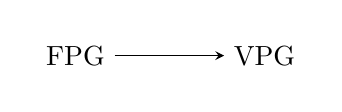
\begin{tikzpicture}
\matrix (m) [matrix of math nodes,row sep=4em,column sep=4em,minimum width=2em]
{
	\text{FPG} & \text{VPG} \\
};
\path[-stealth]
(m-1-1)
edge (m-1-2);
\end{tikzpicture}\\
To do so we have to translate products to configuration, which is trivial, furthermore we have to make the FPG deadlock free. This is done by creating two losing vertices $l_0$ and $l_1$ such that player $\alpha$ loses when the token is in vertex $l_\alpha$. Any vertex that can not move for a configuration will get an edge that is admissible for that configuration towards one of the losing vertices.
\begin{definition}
	\label{def_FPG2VPG}
	FPG2VPG($G^F$) converts FPG $G^F = (V^F, V_0^F, V_1^F, E^F, \rho^F, N, P, \gamma)$ to VPG $G = (V, V_0, V_1, E, \rho, \mathfrak{C}, \theta)$.
	
	Let $P$ be defined as  $\{p_0, p_1, \dots, p_m\}$, we define $\mathfrak{C} = \{c_0, c_1, \dots, c_m\}$.
	
	We create vertices $l_0$ and $l_1$ and define $V_0 = V_0^F \cup \{l_0\}$, $V_1 = V_1^F \cup \{l_1\}$ and $V = V_0 \cup V_1$.
	
	We construct $E$ by first making $E = E^F$ and adding edges $(l_0, l_0)$ and $(l_1, l_1)$ to $E$. Simultaneously we construct $\theta$ by first making $\theta(e) = \{c_i \in \mathfrak{C} | p_i \models \gamma(e)\}$ for every $e \in E^F$. Furthermore $\theta(l_0,l_0) = \theta(l_1,l_1) = \mathfrak{C}$.
	
	Next, for every vertex $v \in V_\alpha$ with $\alpha = \{0,1\}$, we have $C = \mathfrak{C} \backslash \bigcup \{\theta(v,w)|(v,w) \in E\}$. If $C \neq \emptyset$ then we add $(v, l_\alpha)$ to $E$ and make $\theta(v,l_\alpha) = C$.
	Finally we have 
	\[ \rho(v) = \begin{cases}
	1  & \text{if } v = l_0 \\
	0 & \text{if } v = l_1 \\
	\rho^F(v) &\text{otherwise}
	\end{cases} \]
\end{definition}
Again considering our previous working example we can translate the FPG shown in figure \ref{fig:exverfpg} to the VPG shown in figure \ref{fig:exvevpg}. Where $c_0$ corresponds to product $\emptyset$, $c_1$ corresponds to $\{f\}$ and $c_2$ to $\{f,g\}$.
\begin{figure}[h]
	\centering
	\includegraphics[scale=0.3]{Examples/ExamleVerification/VPG}
	\caption[VPG]{VPG}
	\label{fig:exvevpg}
\end{figure}

\subsection{FTS verification using VPG}
We have shown in theorem \ref{the_FPG_ver_FTS} that we can use an FPG to verify an FTS. Next we will show that a winning set in the FPG $M$ is the subset of the winning set in the VPG $FPG2VPG(M)$.
\begin{theorem}
	\label{the_FPG_sub_VPG}
	Given:
	\begin{itemize}
		\item FPG $G^F = (V^F, V_0^F, V_1^F, E^F, \rho^F, N, \{p_0, p_1, \dots, p_m\}, \gamma)$,
		\item product $p_i$
	\end{itemize}
	we have for winning sets $W_\alpha^{p_i}$ in $G$ and $W_\alpha^{c_i}$ in FPG2VPG($G^F$) that $W_\alpha^{p_i} \subseteq W_\alpha^{c_i}$ for any $\alpha \in \{0,1\}$.
	\begin{proof}
		Let $G = (V,V_0,V_1, E, \rho, \mathfrak{C},\theta) =$ FPG2VPG($G^F$). Consider finite play $\pi$ that is valid in game $G^F$ for product $p_i$. We have for every $(\pi_i, \pi_{i+1})$ in $\pi$ that $(\pi_i, \pi_{i+1}) \in E^F$ and $p_i \models \gamma((\pi_i, \pi_{i+1}))$. From the $FPG2VPG$ definition (\ref{def_FPG2VPG}) it follows that $(\pi_i, \pi_{i+1}) \in E$ and $c_i \in \theta(\pi_i, \pi_{i+1})$. So we can conclude that path $\pi$ is also valid in game $G$ for configuration $c_i$. Since the play is finite the winner is determined by the last vertex $v$ in $\pi$, player $\alpha$ wins such that $v \in V_{\overline{\alpha}}$. Furthermore we know, because the play is finite, that there exists no $(v,w) \in E^F$ with $p \models \gamma(v,w)$. From this we can conclude that $(v, l_{\overline{\alpha}}) \in E$ and $c_i \in \theta(v, l_{\overline{\alpha}})$. Vertex $l_{\overline{\alpha}}$ has one outgoing edge, namely to itself. So finite play $\pi$ will in game $G^F$ results in an infinite play $\pi(l_{\overline{\alpha}})^\omega$. Vertex $l_{\overline{\alpha}}$ has a priority with the same parity as player $\alpha$, so player $\alpha$ wins the infinite play in $G$ for configuration $c_i$.
		
		Consider infinite play $\pi$ that is valid in game $G^F$ for product $p_i$. As shown above this play is also valid in game $G$ for configuration $c_i$. Since the win conditions of both games are the same the play will result in the same winner.
		
		Consider infinite play $\pi$ that is valid in game $G$ for configuration $c_i$. We distinguish two cases:
		\begin{itemize}
			\item If $l_\alpha$ doesn't occur in $\pi$ then the path is also valid for game $G^F$ with product $p_i$ and has the same winner.
			\item If $\pi = \pi'(l_\alpha)^\omega$ with no occurrence $l_\alpha$ in $\pi'$ then the winner is player $\overline{\alpha}$. The path $\pi'$ is valid for game $G^F$ with product $p_i$. Let vertex $v$ be the last vertex of $\pi'$. Since $(v, l_\alpha) \in E$ and $c_i \in \theta(v,l_\alpha)$ we know that there is no $(v,w) \in E^F$ with $p_i \models \gamma(v,w)$ and that vertex $v$ is owned by player $\alpha$. So in game $G^F$ player $\alpha$ can't move at vertex $v$ and therefore loses the game (in which case the winner is also $\overline{\alpha}$.
		\end{itemize}
		
		We have shown that every path (finite or infinite) in game $G^F$ with product $p_i$ can be played in game $G$ with configuration $c_i$ and that they have the same winner. Furthermore every infinite path in game $G$ with configuration $c_i$ can be either played as an infinite path or the first part of the path can be played in $G^F$ with product $p_i$ and they have the same winner. From this we can conclude that the theorem holds.
	\end{proof}
\end{theorem}
We can conclude the diagram depicting the relation between the different games and transition systems:\\
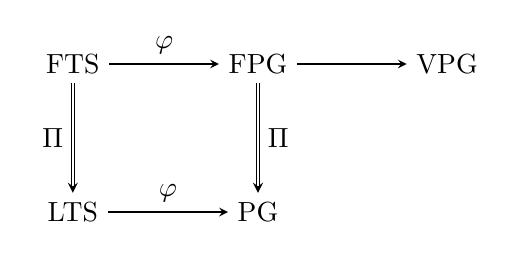
\begin{tikzpicture}
\matrix (m) [matrix of math nodes,row sep=4em,column sep=4em,minimum width=2em]
{
	\text{FTS} & \text{FPG} & \text{VPG} \\
	\text{LTS} & \text{PG} \\};
\path[-stealth]
(m-1-1) edge [double] node [left] {$\Pi$} (m-2-1)
edge node [above] {$\varphi$} (m-1-2)
(m-2-1.east|-m-2-2) edge node [above] {$\varphi$}
(m-2-2)
(m-1-2) edge [double] node [right] {$\Pi$} (m-2-2)
edge (m-1-3);
\end{tikzpicture}\\
Finally we show that VPGs can be used to verify FPGs.
\begin{theorem}
	\label{the_VPG_ver_FTS}
	Given:
	\begin{itemize}
		\item FTS $M = (S, Act, trans, s_0, N, \{p_0,\dots,p_m\}, \gamma)$,
		\item closed modal mu-calculus formula $\varphi$,
		\item product $p_i \in P$ and
		\item state $s \in S$
	\end{itemize}
	it holds that $M_{|p_i}, s \models \varphi$ if and only if $(s, \varphi) \in W_0^{c_i}$ in $FPG2VPG(FTS2FPG(M, \varphi))$.
	\begin{proof}
		Using theorem \ref{the_FPG_ver_FTS} we find that $M_{|p_i}, s \models \varphi$ if and only if $(s, \varphi) \in W_0^{p_i}$ for game $FTS2FPG(M, \varphi)$. If $(s, \varphi) \in W_0^{p_i}$ then we find by using theorem \ref{the_FPG_sub_VPG} that $(s, \varphi) \in W_0^{c_i}$ for game $FPG2VPG(FTS2FPG(M, \varphi))$. If $(s, \varphi) \not\in W_0^{p_i}$ then $(s, \varphi) \in W_1^{p_i}$ and therefore $(s, \varphi) \in W_1^{c_i}$ for game $FPG2VPG(FTS2FPG(M, \varphi))$ and $(s, \varphi) \not\in W_0^{c_i}$.
	\end{proof}
\end{theorem}
This theorem concludes the model verification technique depicted in figure \ref{fig:ftsverificationusingvpg}.

\subsection{Variability parity games}


\subsection{Creating parity games}
Originating from an FTS and a modal $\mu$-calculus we can create an FPG (from which we can create a PG by projection) and from the FPG we can create a VPG. For a specific product we can project the FTS to an LTS, from which we can create a PG. The relation between the transition systems and games is displayed in the following diagram.
\\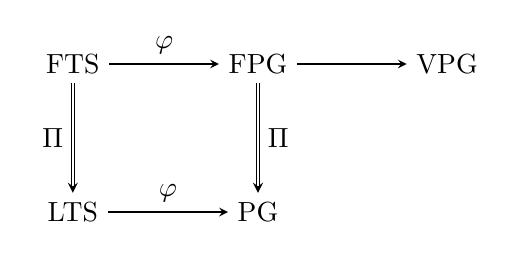
\begin{tikzpicture}
\matrix (m) [matrix of math nodes,row sep=4em,column sep=4em,minimum width=2em]
{
	\text{FTS} & \text{FPG} & \text{VPG} \\
	\text{LTS} & \text{PG} \\};
\path[-stealth]
(m-1-1) edge [double] node [left] {$\Pi$} (m-2-1)
edge node [above] {$\varphi$} (m-1-2)
(m-2-1.east|-m-2-2) edge node [above] {$\varphi$}
 (m-2-2)
(m-1-2) edge [double] node [right] {$\Pi$} (m-2-2)
edge (m-1-3);
\end{tikzpicture}\\
The projections are defined in the previous section. In this section we will define the horizontal arrows in the diagram. First we show how to create a PG from an LTS and a  modal $\mu$-calculus formula, this part is well studied and the approach is based on \cite{Bradfield2018}.


\begin{definition}
	\label{def_LTS2PG}\cite{Bradfield2018}
	LTS2PG($M, \varphi$) converts LTS $M = (S, Act, trans, s_0)$ and closed formula $\varphi$ to a PG $(V, V_0, V_1, E, \rho)$.
	
	A vertex in the parity game is represented by a pair $(s, \psi)$ where $s \in S$ and $\psi$ is a modal $\mu$-calculus formula. We will create a vertex for every state with every subformula of $\varphi$ except subformula's of the form $X$. Furthermore we create a vertex for every state with the unfolding of every fixpoint formula. Formally we define the set of vertices by first defining the set of subformula's:
	\[ F = \{ \psi\ |\ \psi \text{ is a subformula of } \varphi \} \text{, note that $\varphi$ is a subformula of $\varphi$,} \]
	the set of subformula's that are of the form $X$:
	\[ F_X = \{ \psi \in F\ |\ \psi = X\} \]
	and the set of unfolded fixedpoint subformula's:
	 \[ F_\sigma = \{\psi[X:=\sigma X. \psi]\ |\ \sigma X. \psi \in F \text{ with } \sigma \in \{\mu, \nu\}\} \]
	Having these sets we can define the set of vertices by:
	\[ V = S \times (F \backslash F_X \cup F_{\sigma})\]
	
	We create the parity game with the smallest set $E$ such that:
	\begin{itemize}
		\item $V = V_0 \cup V_1$,
		\item $V_0 \cap V_1 = \emptyset$ and
		\item for every $v = (s, \psi) \in V$ we have:
		\begin{itemize}
			\item If $\psi = \top$ then $v \in V_1$.
			\item If $\psi = \bot$ then $v \in V_0$.
			\item If $\psi = \psi_1 \vee \psi_2$ then:
				\subitem $v \in V_0$,
				\subitem $(v, (s,\psi_1)) \in E$ and
				\subitem $(v, (s,\psi_2)) \in E$.
			\item If $\psi = \psi_1 \wedge \psi_2$ then:
				\subitem $v \in V_1$,
				\subitem $(v, (s,\psi_1)) \in E$ and
				\subitem $(v, (s,\psi_2)) \in E$.
			\item If $\psi = \langle a \rangle \psi_1$ then $v \in V_0$ and for every $s \xrightarrow{ a} s'$ we have $(v, (s', \psi_1)) \in E$.
			\item If $\psi = [ a ] \psi_1$ then $v \in V_1$ and for every $s \xrightarrow{ a} s'$ we have  $(v, (s', \psi_1)) \in E$.
			\item If $\psi = \mu X. \psi_1$ then $(v, (s, \psi_1[X:=\mu X. \psi_1])) \in E$.
			\item If $\psi = \nu X. \psi_1$ then $(v, (s, \psi_1[X:=\nu X. \psi_1])) \in E$.
		\end{itemize}
	Note that since $\varphi$ is closed and we use unfolding there will never be an edge $(v,(s, X)) \in E$.
	\end{itemize}


Finally we have $\rho(s, \psi) = \begin{cases}
2 \lfloor adepth(X) / 2 \rfloor & \text{if } \psi = \nu X. \psi'\\
2 \lfloor adepth(X) / 2 \rfloor + 1 & \text{if } \psi = \mu X. \psi'\\
0 & \text{otherwise}
\end{cases}$
\end{definition}
Next we define the transformation from FTS to FPG.
\begin{definition}
	\label{def_FTS2FPG}
	FTS2FPG($M, \varphi$) converts FTS $M = (S, Act, trans, s_0, N, P, \gamma)$ and closed formula $\varphi$ to FPG $(V, V_0, V_1, E, \rho, N, P, \gamma')$.
	
	We have $(V, V_0, V_1, E, \rho)$ = LTS2PG($(S, Act, trans, s_0), \varphi$) and
	\[ \gamma'((s, \psi),(s', \psi')) = \begin{cases}
	\gamma(s,a,s') & \text{if }\psi = \langle a \rangle \psi'\text{ or }\psi = [a]\psi' \\
	\top & \text{otherwise}
	\end{cases}\]
\end{definition}
Finally we define how to create a VPG from an FPG. This transformation abstracts from the notion of products and uses configurations for a syntactically more pleasant representation. Furthermore in VPGs deadlocks are removed, this is done by creating two losing vertices $l_0$ and $l_1$ such that player $\alpha$ loses when the token is in vertex $l_\alpha$. Any vertex that can not move for a configuration will get an edge that is admissible for that configuration towards one of the losing vertices.
\begin{definition}
	\label{def_FPG2VPG}
	FPG2VPG($G^F$) converts FPG $G^F = (V^F, V_0^F, V_1^F, E^F, \rho^F, N, P, \gamma)$ to VPG $G = (V, V_0, V_1, E, \rho, \mathfrak{C}, \theta)$.
	
	Let $P$ be defined as  $\{p_0, p_1, \dots, p_m\}$, we define $\mathfrak{C} = \{c_0, c_1, \dots, c_m\}$.
	
	We create vertices $l_0$ and $l_1$ and define $V_0 = V_0^F \cup \{l_0\}$, $V_1 = V_1^F \cup \{l_1\}$ and $V = V_0 \cup V_1$.
	
	We construct $E$ by first making $E = E^F$ and adding edges $(l_0, l_0)$ and $(l_1, l_1)$ to $E$. Simultaneously we construct $\theta$ by first making $\theta(e) = \{c_i \in \mathfrak{C} | p_i \models \gamma(e)\}$ for every $e \in E^F$. Furthermore $\theta(l_0,l_0) = \theta(l_1,l_1) = \mathfrak{C}$.
	
	Next, for every vertex $v \in V_\alpha$ with $\alpha = \{0,1\}$, we have $C = \mathfrak{C} \backslash \bigcup \{\theta(v,w)|(v,w) \in E\}$. If $C \neq \emptyset$ then we add $(v, l_\alpha)$ to $E$ and make $\theta(v,l_\alpha) = C$.
	Finally we have 
	\[ \rho(v) = \begin{cases}
	1  & \text{if } v = l_0 \\
	0 & \text{if } v = l_1 \\
	\rho^F(v) &\text{otherwise}
	\end{cases} \]
\end{definition}

\subsection{Correctness}


\begin{theorem}
	\label{the_FPG_ver_FTS}
	Given:
	\begin{itemize}
		\item FTS $M = (S, Act, trans, s_0, N, P, \gamma)$,
		\item closed modal mu-calculus formula $\varphi$,
		\item product $p \in P$ and
		\item state $s \in S$
	\end{itemize}
it holds that $M_{|p}, s \models \varphi$ if and only if $(s, \varphi) \in W_0^p$ in FTS2FPG($M, \varphi$).
\begin{proof}
	The winning set $W_\alpha^p$ is equal to winning set $W_\alpha$ in FTS2FPG($M, \varphi$)$_{|p}$ using definition \ref{def_FPG}. Using theorem \ref{the_PGsubPGA} we find that the game FTS2FPG($M, \varphi$)$_{|p}$ is equal to the game LTS2PG($M_{|p}, \varphi$), obviously their winning sets are also equal. Using the modal verification proof from \cite{Bradfield2018} we know that $M_{|p}, s \models \varphi$ if and only if $(s, \varphi) \in W_0$. Winning set $W_\alpha^p$ is equal to $W_\alpha$, therefore the theorem holds.
\end{proof}
\end{theorem}

\begin{theorem}
	\label{the_FPG_sub_VPG}
	Given:
	\begin{itemize}
		\item FPG $G^F = (V^F, V_0^F, V_1^F, E^F, \rho^F, N, \{p_0, p_1, \dots, p_m\}, \gamma)$,
		\item product $p_i$,
		\item player $\alpha \in \{0,1\}$
	\end{itemize}
we have for winning sets $W_\alpha^{p_i}$ in $G$ and $W_\alpha^{c_i}$ in FPG2VPG($G^F$) that $W_\alpha^{p_i} \subseteq W_\alpha^{c_i}$.
\begin{proof}
	Let $G = (V,V_0,V_1, E, \rho, \mathfrak{C},\theta) =$ FPG2VPG($G^F$). Consider finite play $\pi$ that is valid in game $G^F$ for product $p_i$. We have for every $(\pi_i, \pi_{i+1})$ in $\pi$ that $(\pi_i, \pi_{i+1}) \in E^F$ and $p_i \models \gamma((\pi_i, \pi_{i+1}))$. From definition \ref{def_FPG2VPG} it follows that $(\pi_i, \pi_{i+1}) \in E$ and $c_i \in \theta(\pi_i, \pi_{i+1})$. So we can conclude that path $\pi$ is also valid in game $G$ for configuration $c_i$. Since the play is finite the winner is determined by the last vertex $v$ in $\pi$, player $\alpha$ wins such that $v \in V_{\overline{\alpha}}$. Furthermore we know, because the play is finite, that there exists no $(v,w) \in E^F$ with $p \models \gamma(v,w)$. From this we can conclude that $(v, l_{\overline{\alpha}}) \in E$ and $c_i \in \theta(v, l_{\overline{\alpha}})$. Vertex $l_{\overline{\alpha}}$ has one outgoing edge, namely to itself. So finite play $\pi$ will in game $G^F$ results in an infinite play $\pi(l_{\overline{\alpha}})^\omega$. Vertex $l_{\overline{\alpha}}$ has a priority with the same parity as player $\alpha$, so player $\alpha$ wins the infinite play in $G$ for configuration $c_i$.
	
	Consider infinite play $\pi$ that is valid in game $G^F$ for product $p_i$. As shown above this play is also valid in game $G$ for configuration $c_i$. Since the win conditions of both games are the same the play will result in the same winner.
	
	Consider infinite play $\pi$ that is valid in game $G$ for configuration $c_i$. We distinguish two cases:
	\begin{itemize}
		\item If $l_\alpha$ doesn't occur in $\pi$ then the path is also valid for game $G^F$ with product $p_i$ and has the same winner.
		\item If $\pi = \pi'(l_\alpha)^\omega$ then the winner is player $\overline{\alpha}$. The path $\pi'$ is valid for game $G^F$ with product $p_i$. Let vertex $v$ be the last vertex of $\pi'$. Since $(v, l_\alpha) \in E$ and $c_i \in \theta(v,l_\alpha)$ we know that there is no $(v,w) \in E^F$ with $p_i \models \gamma(v,w)$ and that vertex $v$ is owned by player $\alpha$. So in game $G^F$ player $\alpha$ can't move at vertex $v$ and therefore loses the game (in which case the winner is also $\overline{\alpha}$.
	\end{itemize}

We have shown that every path (finite or infinite) in game $G^F$ with product $p_i$ can be played in game $G$ with configuration $c_i$ and that they have the same winner. Furthermore every infinite path in game $G$ with configuration $c_i$ can be either played as an infinite path or the first part of the path can be played in $G^F$ with product $p_i$ and they have the same winner. From this we can conclude that the theorem holds.
\end{proof}
\end{theorem}
\bibliography{mybib} 
\bibliographystyle{ieeetr}

\end{document}
